\subsubsection{ln 3}\label{sssec:ln3}\index{ln3@$\ln3$}
 
\zadatak
У част Непера и Бригса,
помоћу поступка \eqref{eq:alg}\index{алгоритам} са 
стране~\pageref{eq:alg},
израчунај {\sl пешке\/} приближну вредност $\ln 3$\index{бројна вредност}
у~5 корака. За упоређивање, тачна вредност је
$$
\ln3=1\.
0986122886\,
6810969139\,
5245236922\,
5257046475\,\ldots
%1639157/1492025=1.098612288668
$$

\def\step#1{\par\indent\leavevmode
  Корак~{\it#1}.\kern2em\relax}

\resenje
За $x=3$ биће $r=(x-1)/(x+1)=1/2$. У нултом кораку постављамо почетне вредности:

\smallskip

\step0 $k=1,\quad p=2r=1,\quad q=r^2=1/4,\quad a=p=1,\quad y=a=1$.

\smallskip

\noindent Следе кораци итерације --- повећамо $k$ за 2, помножимо $p$ са $q$,
члан суме $a$ постаје $p/k$, кога додајемо у резултат $y$:

\smallskip

\step1 $k=3,\quad p=1/4,\quad a=1/12,\quad y=13/12$;
\step2 $k=5,\quad p=1/16,\quad a=1/80,\quad y=263/240$;
\step3 $k=7,\quad p=1/64,\quad a=1/448,\quad y=7379/6720$;
\step4 $k=9,\quad p=1/256,\quad a=1/2304,\quad y=88583/80640$;
\step5 $k=11,\quad p=1/1024,\quad a=1/11264,\quad y=3897967/3548160$.

\smallskip

\noindent Резултат је
$$
\ln3\approx\frac{3897967}{3548160}=
\ram{1.098588\ldots} 
% \ram{1\.0986},
$$
што није лоше за само 5 корака, јер је апсолутна грешка око $2\.4\puta10^{-5}$.
Али \dots, може боље.

\dodatak
Ако већ имамо прецизно израчунату вредност $\ln2$\index{ln2@$\ln 2$}, онда је боље рачунати $\ln3$ као $\ln(3/4)+2\ln2$,
јер ће, уместо $r=1/2$, бити $r=(3/4-1)/(3/4+1)=-1/7$, 
односно, уместо $q=1/4$, биће $q=1/49$,
што доводи до много бржег израчунавања. У~истом броју корака бисмо добили
$$
\ln\frac34\approx
-\ff2/7, -\ff296/1029, -\ff72526/252105, -\ff24876448/86472015, 
-\ff522405418/1815912315, -\ff281576520392/978776737785,
$$
где последњи разломак има грешку од око $1\.6\puta10^{-12}$,
што је више од двоструко тачних цифара.
Када му (са стране~\pageref{eq:ln2}) додамо $2\ln2$, добићемо
$$
\ln3\approx 2\ln2 -\frac{281576520392}{978776737785} =
{\,\underbrace{\!1\.0986122886\,6\!}_{\hbox{\scriptsize 12 тачних цифара}}972615081\,\ldots}
$$

Уопштено, поступак је најбржи ако рачунамо $\ln x=\ln(x/2^n)+n\ln2$,\index{ln@$\ln$}
где бирамо $n$ такво да $x/2^n$ буде што ближе 1, односно, да $q$ буде најмање могуће (види \idx{програм}).%
\index{компјутер}\index{ZX Spectrum@\textsf{ZX Spectrum}}\index{BASIC@\BASIC}\index{епсилон $(\varepsilon)$}%
$$
\slika{\hbox to \textwidth{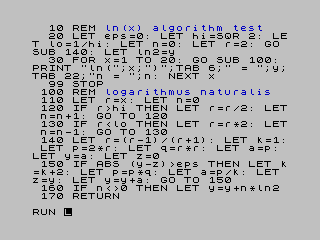
\includegraphics[width=\zxscreen]{ln-prog.png}\hss
  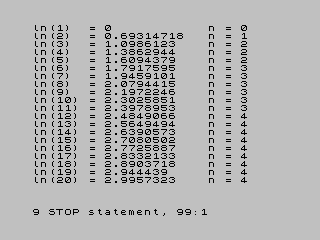
\includegraphics[width=\zxscreen]{ln-run.png}}}{\href{https://fuse-emulator.sourceforge.net/}{\textsf{ZX Spectrum}} \href{\GitHubRaw ln.z80}{\BASIC} програм.}
$$
